\documentclass{beamer}
\usetheme[faculty=econ]{fibeamer}

\usepackage[utf8]{inputenc}
\usepackage[francais]{babel}
\usepackage[T1]{fontenc}
\usepackage{xcolor}

\lstset{
  language=Java,                
  basicstyle=\scriptsize,
  escapeinside={*@}{*@},
  frame=single,
  xleftmargin=2mm,
  xrightmargin=2mm,
  keepspaces=true,
  tabsize=2
}

\newcounter{ctr1}
\title[]{\Large{Développement d'applications modulaires en Java}}
\author[C. Tibermacine]{\large{Chouki~Tibermacine}\\
\small{Chouki.Tibermacine@umontpellier.fr}}
%\institute{Polytech Montpellier}
\date{}

\begin{document}

\begin{frame}
\titlepage
\begin{flushright}

\includegraphics[width=3.5cm]{figs/polytech.png}
\end{flushright}
\end{frame}

\begin{frame}
	\frametitle{Plan de l'ECUE}
	\begin{enumerate}
		{\color{gray}{\item (Rappels sur le) Développement d'applications Web avec Java
				\item Modulariser les applications Java avec Spring
				\item Bien structurer une application Web avec Spring MVC
				\item Auto-configurer une application Web avec Spring Boot
				\item Sécuriser une application Web avec Spring Security
		\item Gérer des données massives avec Apache Kafka et Spring}}
						\item Tester une application Web Spring
{\color{gray}{				\item Écrire des applications Web (API) réactives avec Spring WebFlux}}
	\end{enumerate}
\end{frame}

\AtBeginSection[]{% Print an outline at the beginning of sections
  \begin{frame}<beamer>
    \frametitle{Plan du cours}
    % \frametitle{Outline}
    \tableofcontents[currentsection]
    % \tableofcontents
  \end{frame}}

\AtBeginSubsection[]{% Print an outline at the beginning of sections
  \begin{frame}<beamer>
    \frametitle{Plan du cours}
    % \frametitle{Outline}
    \tableofcontents[currentsubsection]
    % \tableofcontents
  \end{frame}}

\section{Automatisation des tests en Java avec JUnit}

\begin{frame}
	\frametitle{Premiers tests automatisés en Java}
	\begin{itemize}
		\item Je vous invite à consulter d'abord le cours sur les assertions et JUnit, disponible dans le dépôt Git
		\item C'est un cours de prog par objets
		\item Si vous n'avez pas beaucoup pratiqué les tests avant ce cours, lisez attentivement le contenu du cours, et réalisez les exemples
		\item Sinon, parcourez rapidement les diapos du cours et passez à la suite de ce cours
	\end{itemize}
\end{frame}

\section{Introduction aux tests avec Spring}

\begin{frame}
  \frametitle{Tests dans une application Web}
  \begin{itemize}
  \item Vous avez probablement remarqué le dossier \texttt{test} créé par Spring Initializr ou par l'IDE pour votre projet Gradle
  \item Ce dossier comporte une classe qui porte le nom de votre projet + \texttt{ApplicationTests}
  \item Cette classe est annotée \texttt{@SpringBootTest}
  \item Cette annotation indique à Spring Boot qu'il faut rechercher une classe principale de configuration (annotée \texttt{@SpringBootApplication}, par ex) et l'utiliser pour démarrer/créer le contexte de l'application (tous les objets qui composent l'application : contrôleurs, modèles, ...)
  \item La classe de test comporte des méthodes de test (cas de tests)
  \item On peut définir plusieurs classes de test annotées de cette façon
\end{itemize}
\end{frame}

\begin{frame}[fragile]
	\frametitle{Un premier test Spring}
	Modifier la classe en~:
	\begin{itemize}
		\item ajoutant un attribut auto-injecté par une référence à l'un de vos contrôleurs. Par exemple~:
\begin{lstlisting}
@Autowired
private HomeController controller;
\end{lstlisting}
		\item Dans la méthode de test ajouter une assertion~:
\begin{lstlisting}
@Test
public void contextLoads() throws Exception {
	assertThat(controller).isNotNull();
}
\end{lstlisting}
Ajouter un import statique des méthodes \texttt{assertXxx()}~:
\begin{lstlisting}
import static org.assertj.core.api.Assertions.*;
\end{lstlisting}
	\end{itemize}
\end{frame}

\begin{frame}[fragile]
	\frametitle{Exécuter le test}
	\begin{itemize}
		\item Démarrer le test en exécutant la tâche \texttt{verification/test} (tool-window Gradle à droite), ou bien clique bouton droit sur la méthode puis \texttt{Run}
		\item Vous allez voir le test passer au vert
		\item C'est normal, parce que le contrôleur est bien instancié par Spring Boot lors de la création du contexte de l'application
		\item L'étape suivante est de tester le comportement de l'app Web
		\item Tester l'envoi d'une requête HTTP et vérifier le contenu de la réponse (voir diapo suivante)
	\end{itemize}
\end{frame}

\begin{frame}[fragile]
	\frametitle{Classe de test d'une requête HTTP}
\begin{lstlisting}
@SpringBootTest(webEnvironment = WebEnvironment.RANDOM_PORT)
public class HttpRequestTest {
	
	@LocalServerPort
	private int port;
	
	@Autowired
	private TestRestTemplate restTemplate;
	
	@Test
	public void greetingShouldReturnDefaultMessage() throws Exception {
		assertThat(this.restTemplate.getForObject("http://localhost:" + port + "/",
		String.class)).contains("Hello, World");
	}
}
\end{lstlisting}
\end{frame}

\begin{frame}[fragile]
	\frametitle{Classe de test d'une requête HTTP -suite-}
	Plusieurs facilités offertes par Spring, utilisées dans l'exemple précédent~:
	\begin{itemize}
		\item L'utilisation de \texttt{webEnvironment=RANDOM\_PORT} permet le démarrage du serveur avec un port aléatoire (utile pour éviter les conflits de ports dans un environnement de tests)
		\item L'injection du port avec l'annotation \texttt{@LocalServerPort}
		\item L'attribut de type \texttt{TestRestTemplate} permet de tester l'envoi de requêtes HTTP~; il a été auto-injecté avec \texttt{Autowired} (bean disponible grâce à l'annotation \texttt{@SpringBootTest})
	\end{itemize}
\end{frame}

\begin{frame}
	\frametitle{Surcoût de démarrer un serveur Web}
	\begin{itemize}
		\item Pour éviter le surcoût induit par un serveur Web, on peut utiliser Spring MockMvc
		\item Ceci permet de tester tout ce qu'il y a derrière le serveur Web comme application, mais sans devoir démarrer le serveur
		\item Il suffit d'ajouter l'annotation suivante à la classe de test~: \texttt{@AutoConfigureMockMvc}
	\end{itemize}
\end{frame}

\begin{frame}[fragile]
	\frametitle{Exemple avec Spring MockMvc}
\begin{lstlisting}
@SpringBootTest
@AutoConfigureMockMvc
public class TestingWebApplicationTest {
	
 @Autowired
 private MockMvc mockMvc;

 @Test
 public void shouldReturnDefaultMessage() throws Exception {
  this.mockMvc.perform(get("/")).andDo(print())
  .andExpect(status().isOk())
  .andExpect(content()
   .string(containsString("Hello, World")));
 }
}
\end{lstlisting}
Ceci permet de démarrer tout le contexte d'application Spring (tous ses objets), mais pas le serveur
\end{frame}

\begin{frame}[fragile,label={webmvc}]
	\frametitle{Exemple avec Spring WebMvcTest}
	\begin{itemize}
		\item On peut limiter les tests à la couche Web avec \texttt{@WebMvcTest}
	\end{itemize}
\begin{lstlisting}
@WebMvcTest
public class WebLayerTest {
	
 @Autowired
 private MockMvc mockMvc;

 @Test
 public void shouldReturnDefaultMessage() throws Exception {
  this.mockMvc.perform(get("/")).andDo(print())
  .andExpect(status().isOk())
  .andExpect(content().string(
    containsString("Hello, World")));
 }
}
\end{lstlisting}
Noter l'utilisation de \texttt{MockMvc} pour envoyer une requête HTTP, obtenir la réponse et enchaîner avec des assertions sur cette réponse
\end{frame}

\begin{frame}
	\frametitle{Exemple avec Spring WebMvcTest -suite-}
	\begin{itemize}
		\item Dans l'exemple précédent, Spring Boot instancie les objets de la couche Web seulement (pas tout le contexte)
		\item Dans une application avec plusieurs contrôleurs, on peut restreindre les tests à un seul contrôleur avec \texttt{@WebMvcTest(HomeController.class)}
		\item Si le contrôleur a des dépendances vers d'autres objets de l'application (des objets \texttt{@Service}, par exemple, sur lesquels il invoque des méthodes), on doit utiliser un framework pour créer un \textit{Mock} (simulacre) pour les simuler, comme \textit{Mockito}~:
		\footnotesize \url{https://site.mockito.org/}\\
		\normalsize
		Tuto~: 
		\footnotesize
		\url{https://www.vogella.com/tutorials/Mockito/article.html}
		\normalsize
		\item Dans Spring, l'intégration de Mockito est transparente, avec des objets \textit{MockBean} (toute la config de ce framework est faite automatiquement)
	\end{itemize}
\end{frame}

\begin{frame}[fragile]
	\frametitle{Exemple avec intégration de Mockito}
\begin{lstlisting}
@Controller
public class GreetingController {	
 private final GreetingService service;
 public GreetingController(GreetingService service) {
  this.service = service;
 }
 @RequestMapping("/greeting")
 public @ResponseBody String greeting() {
  return service.greet();
 }	
}
\end{lstlisting}
\begin{lstlisting}
@Service
public class GreetingService {
 public String greet() {
  return "Hello, World";
 }
}	
\end{lstlisting}
\end{frame}

\begin{frame}[fragile]
	\frametitle{Exemple avec intégration de Mockito -suite-}
\begin{lstlisting}
@WebMvcTest(GreetingController.class)
public class WebMockTest {	
 @Autowired
 private MockMvc mockMvc;
 @MockBean
 private GreetingService service;	
 @Test
 public void greetingShouldReturnMessageFromService() throws Exception {
  when(service.greet()).thenReturn("Hello, Mock");
  this.mockMvc.perform(get("/greeting")).andDo(print())
  .andExpect(status().isOk()).andExpect(content()
    .string(containsString("Hello, Mock")));
 }
}
\end{lstlisting}
\texttt{GreetingService} est remplacé par un mock (créé et injecté par Spring) dont le comportement est décrit par la 1ère ligne de code de la méthode de test
\end{frame}

\section{Tests unitaires avec un backend SQL}

\begin{frame}
	\frametitle{Stratégie de test pour une app Web Spring}
	Réaliser des tests unitaires pour (dans l'ordre)~:
	\begin{enumerate}
		\item les contrôleurs
		\item les services, le cas échéant
		\item les repositories
	\end{enumerate}
	Ensuite, réaliser des tests d'intégration de ces trois couches
\end{frame}

\begin{frame}
	\frametitle{1. Tester les contrôleurs}
	Utiliser MockMvc tel qu'on l'a vu dans la diapo~{\color{blue}\ref{webmvc}} pour~:
\begin{itemize}
	\item exécuter des requêtes HTTP vers le contrôleur
	\item valider les réponses HTTP
	\item valider les entêtes HTTP
	\item valider les corps des réponses
\end{itemize}
\end{frame}


\begin{frame}[fragile]
	\frametitle{Écrire un test}
	\begin{itemize}

		\item La première partie de la méthode de test (la section \textit{Given} d'un \textit{test case}) comporte la mise en place du Mock~:
\begin{lstlisting}
@WebMvcTest(GreetingController.class)
public class WebMockTest {	
	@Autowired
	private MockMvc mockMvc;
	@MockBean
	private GreetingService service;	
	@Test
	public void greetingShouldReturnMessageFromService() throws Exception {
		when(service.greet()).thenReturn("Hello, Mock");	
		// ...
\end{lstlisting}	
Ici, il faut lire l'instruction de la façon suivante~: quand (\texttt{when}) la méthode \texttt{greet()} est invoquée sur l'objet simulé, celle-ci doit retourner la valeur indiquée en paramètre de \texttt{thenReturn}
		\end{itemize}
\end{frame}

\begin{frame}[fragile]
	\frametitle{Écrire un test -suite-}
	
	\begin{itemize}
		\item La 2ème partie comporte l'exécution de la requête HTTP (\textit{When} d'un test case) et la validation de la réponse~:
\begin{lstlisting}
this.mockMvc.perform(get("/greeting")).andDo(print())
// Verfication du header
.andExpect(status().isOk())
// Verification du contenu
.andExpect(content()
           .string(containsString("Hello, Mock")));		
\end{lstlisting}
\item \texttt{andExpect()} permet de tester une hypothèse (en prenant en paramètre un \textit{result matcher}) et de chaîner les tests
\item status() et content() sont des méthodes importées statiquement du framework Spring Test~:\\
\footnotesize
\texttt{org.springframework.test.web.servlet.result.MockMvcResultMatchers}
\normalsize
\item \texttt{containsString()} provient de Hamcrest (framework de matchers)~:
\footnotesize
\url{http://hamcrest.org/JavaHamcrest/tutorial}
\normalsize
	\end{itemize}
\end{frame}

\begin{frame}[fragile]
	\frametitle{Un exemple plus élaboré - test service REST}
	\begin{tikzpicture}[overlay,remember picture]
		\node[anchor=center,xshift=20pt,yshift=0pt]
		at (current page.center) {
			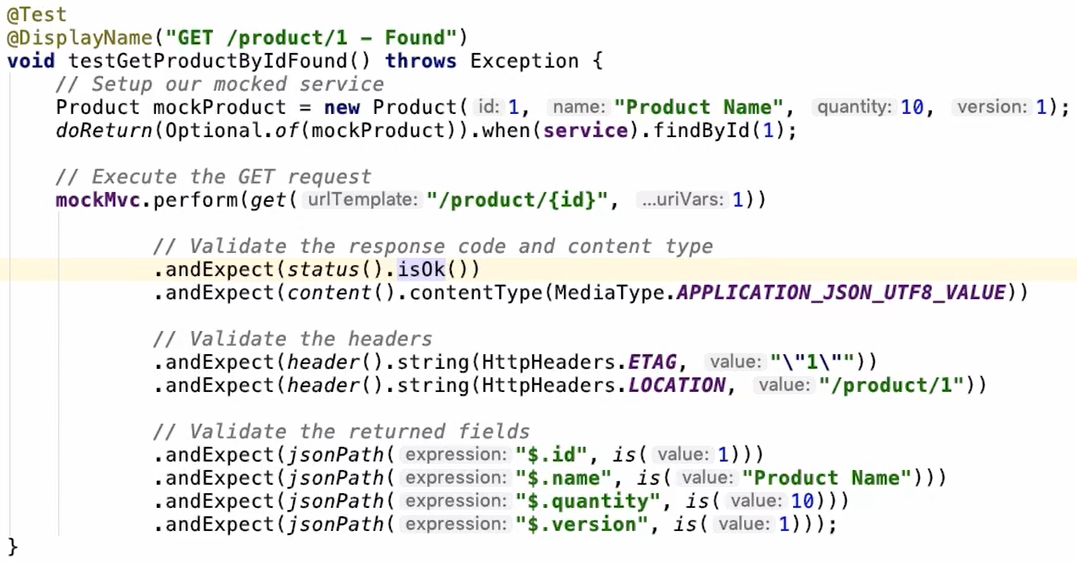
\includegraphics[width=11cm]{img/test_get.png}
		};
	\end{tikzpicture}
\vspace{5.5cm}
\begin{itemize}
	\item[] Ici, \texttt{service} est un service simulé avec le mock. Quand sa méthode findById(1) est invoqué, il doit retourner l'objet \texttt{mockProduct}
\end{itemize}

\end{frame}

\begin{frame}[fragile]
	\frametitle{Dans l'exemple précédent}
	\begin{itemize}
		\item Est-ce que vous avez remarqué le header ETag~?
		\item A quoi sert-il ?
		\item Un header très utile dans la définition d'API REST, notamment pour gérer les versions des ressources (users, locations, ...)
		\item Utile dans la gestion des requêtes PUT (mise à jour d'une ressource) pour détecter les conflits (si jamais lors de la mise à jour, la version d'une ressource a changé depuis le dernier GET (elle a été mise à jour par un autre utilisateur). Il y a donc un conflit : erreur HTTP 409 retourné normalement)
		\item Plus de détails ici~:\\
		\footnotesize
		 \url{https://www.baeldung.com/etags-for-rest-with-spring}
		 \normalsize
	\end{itemize}
\end{frame}

\begin{frame}[fragile]
	\frametitle{Toujours dans l'exemple précédent}
	\begin{itemize}
		\item Est-ce que vous connaissez JsonPath ?
		\item Un langage de requêtes de données JSON (requêtes déclaratives à la manière de XPath)
		\item Un interprète de ce langage est fourni via la méthode jsonPath de \texttt{MockMvcResultMatchers} de Spring
		\item \texttt{\$} dans l'exemple veut dire l'élément racine de la donnée JSON dans la réponse HTTP
		\item Plus de détails sur JsonPath~:\\
		\footnotesize
		\url{https://www.baeldung.com/guide-to-jayway-jsonpath}
		\normalsize
	\end{itemize}
\end{frame}

\begin{frame}[fragile]
	\frametitle{Test service REST - Get Not Found}
	\begin{tikzpicture}[overlay,remember picture]
		\node[anchor=center,xshift=20pt,yshift=20pt]
		at (current page.center) {
			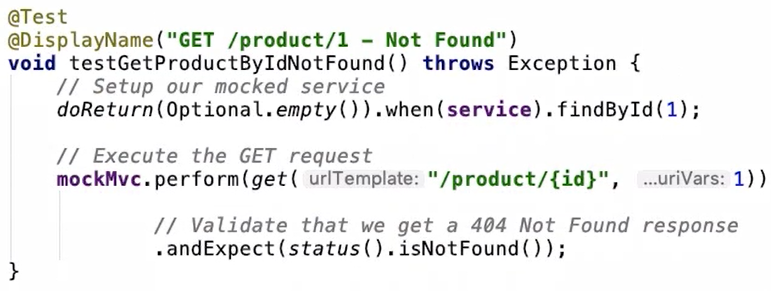
\includegraphics[width=11cm]{img/test_get_not_found.png}
		};
	\end{tikzpicture}
	\vspace{4cm}
	\begin{itemize}
		\item On doit tester le scénario lorsque la requête HTTP réussit, mais aussi lorsque ça ne réussit pas \item Ici, lorsqu'on fait un GET d'un produit qui n'existe pas, on teste qu'on a bien en retour un 404
	\end{itemize}
	
\end{frame}

\begin{frame}[fragile]
	\frametitle{Test service REST - POST qui réussit}
	\begin{tikzpicture}[overlay,remember picture]
		\node[anchor=center,xshift=10pt,yshift=2pt]
		at (current page.center) {
			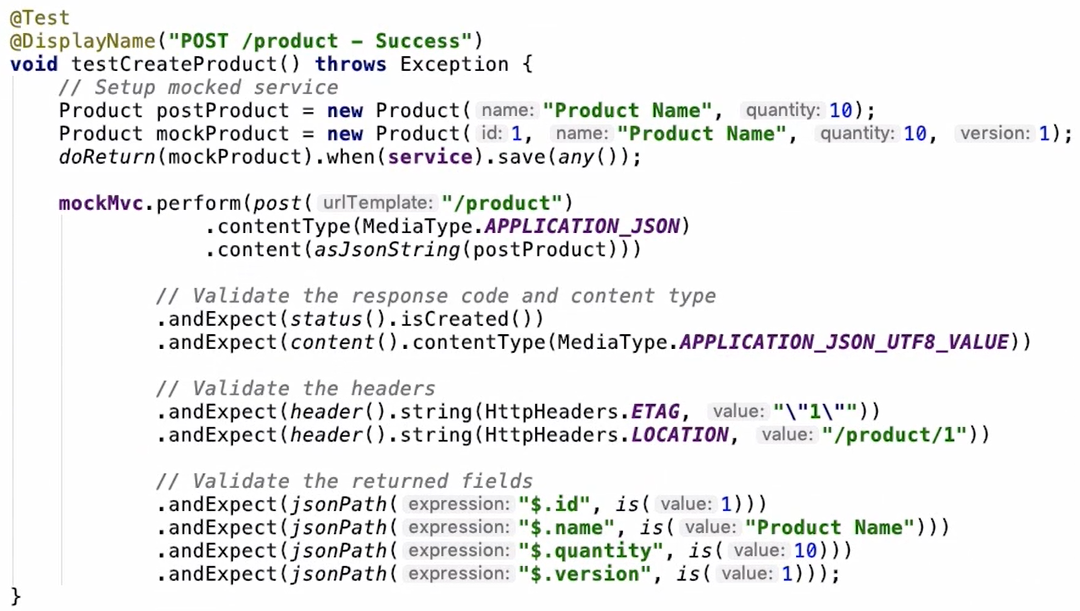
\includegraphics[width=11.5cm]{img/test_post.png}
		};
	\end{tikzpicture}
	\vspace{5.5cm}
	\begin{itemize}
		\item Deux objets ici, l'un passé en paramètre de la requête POST et l'autre utilisé comme Mock
		
	\end{itemize}
	
\end{frame}

\begin{frame}[fragile]
	\frametitle{Dans l'exemple précédent}
	\begin{itemize}
		\item Noter la préparation des données de la requête dans l'invocation à \texttt{perform()}
		\item \texttt{asJsonString()} est une méthode qui n'est pas montrée, mais qui utilise simplement la bibliothèque Jackson pour sérialiser l'objet en JSON (voir diapo~{\color{blue}\ref{obj2json}})
		\item On s'assure ensuite que la réponse a le \textit{status Ok} (HTTP 200)
		\item On vérifie ensuite les headers et le contenu (charge utile) de la réponse
	\end{itemize}
{\color{gray} Des exemples, que vous pouvez copier, sont donnés à la fin du cours}
\end{frame}

\begin{frame}[fragile]
	\frametitle{Test service REST - PUT qui réussit}
	\begin{tikzpicture}[overlay,remember picture]
		\node[anchor=center,xshift=10.5pt,yshift=0pt]
		at (current page.center) {
			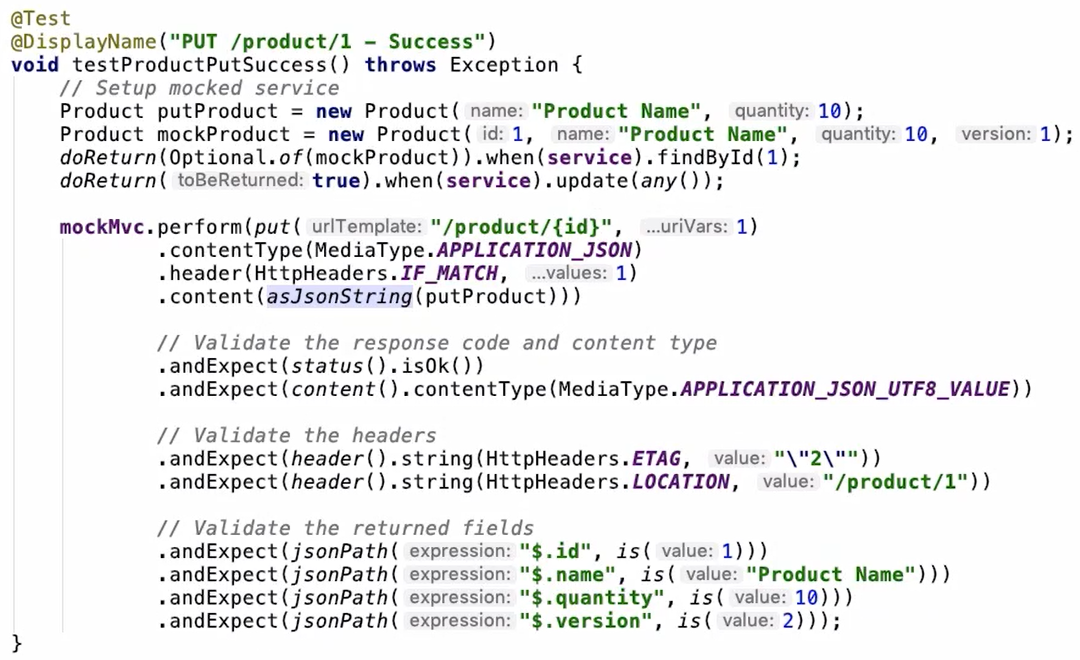
\includegraphics[width=10cm]{img/test_put.png}
		};
	\end{tikzpicture}
	\vspace{5.5cm}
	\begin{itemize}
		\item Là aussi, deux objets sont utilisés (param requête et Mock)
	\end{itemize}	
\end{frame}

\begin{frame}[fragile]
	\frametitle{Dans l'exemple précédent}
	\begin{itemize}
		\item Noter la préparation des données de la requête dans l'invocation à \texttt{perform()} avec cette fois un header \texttt{IF\_MATCH} pour vérifier le ETag
		\item On s'assure que la réponse a le \textit{status Created} (HTTP 201)
		\item On vérifie ensuite les headers et le contenu (charge utile) de la réponse
	\end{itemize}
\end{frame}

\begin{frame}[fragile]
	\frametitle{Test service REST - PUT qui échoue - Conflit}
	\begin{tikzpicture}[overlay,remember picture]
		\node[anchor=center,xshift=10pt,yshift=25pt]
		at (current page.center) {
			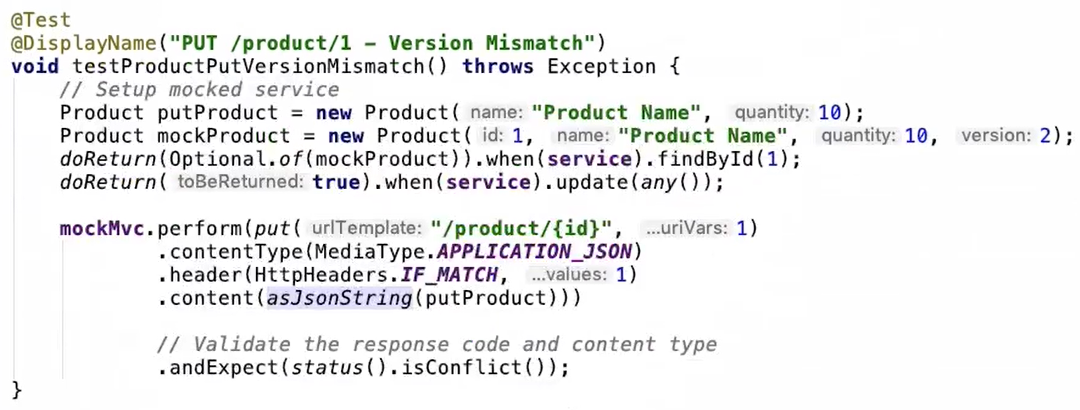
\includegraphics[width=11cm]{img/test_put_nok.png}
		};
	\end{tikzpicture}
	\vspace{3.5cm}
	\begin{itemize}
		\item Noter la valeur de \texttt{IF\_MATCH} (égale à 1) différente de 2 dans l'objet Mock
		\item Le numéro de version est utilisé dans cet exemple come ETag
		\item La réponse attendue doit avoir comme \textit{status Conflict} (HTTP 409) 
	\end{itemize}	
\end{frame}

\begin{frame}[fragile]
	\frametitle{Test service REST - PUT qui échoue - Not Found}
	\begin{tikzpicture}[overlay,remember picture]
		\node[anchor=center,xshift=10pt,yshift=25pt]
		at (current page.center) {
			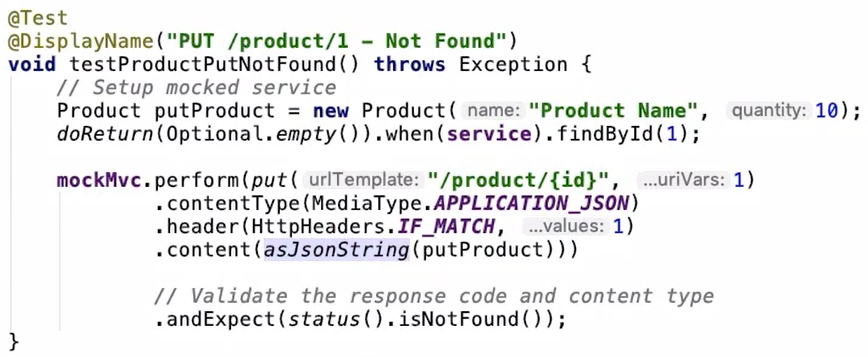
\includegraphics[width=11cm]{img/test_put_not_found.png}
		};
	\end{tikzpicture}
	\vspace{3.5cm}
	\begin{itemize}
		\item Noter la réponse du service simulé par un \texttt{Optional.empty()} (absence de valeur pour simuler une ressource introuvable)
		\item La réponse attendue doit avoir comme \textit{status Not Found} (HTTP 404) 
	\end{itemize}	
\end{frame}

\begin{frame}[fragile]
	\frametitle{Test service REST - DELETE}
	Tester :
	\begin{itemize}
		\item Delete qui réussit (une ressource qui existe)
		\item Delete qui échoue (une ressource qui n'existe pas)
		\item Delete qui échoue (erreur interne, dans la base de données par ex)
	\end{itemize}
\end{frame}

\begin{frame}[fragile]
	\frametitle{Test service REST - DELETE qui réussit}
	\begin{tikzpicture}[overlay,remember picture]
		\node[anchor=center,xshift=10pt,yshift=25pt]
		at (current page.center) {
			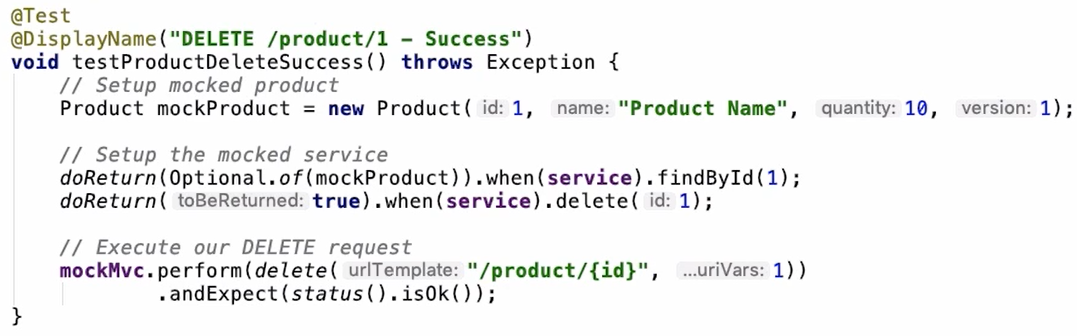
\includegraphics[width=11cm]{img/test_delete.png}
		};
	\end{tikzpicture}
	\vspace{3.5cm}
	\begin{itemize}
		\item On teste simplement le fait que le \textit{status} de la réponse est \textit{Ok}
	\end{itemize}	
\end{frame}

\begin{frame}[fragile]
	\frametitle{Test service REST - DELETE qui échoue}
	\begin{tikzpicture}[overlay,remember picture]
	\node[anchor=center,xshift=10pt,yshift=0pt]
	at (current page.center) {
		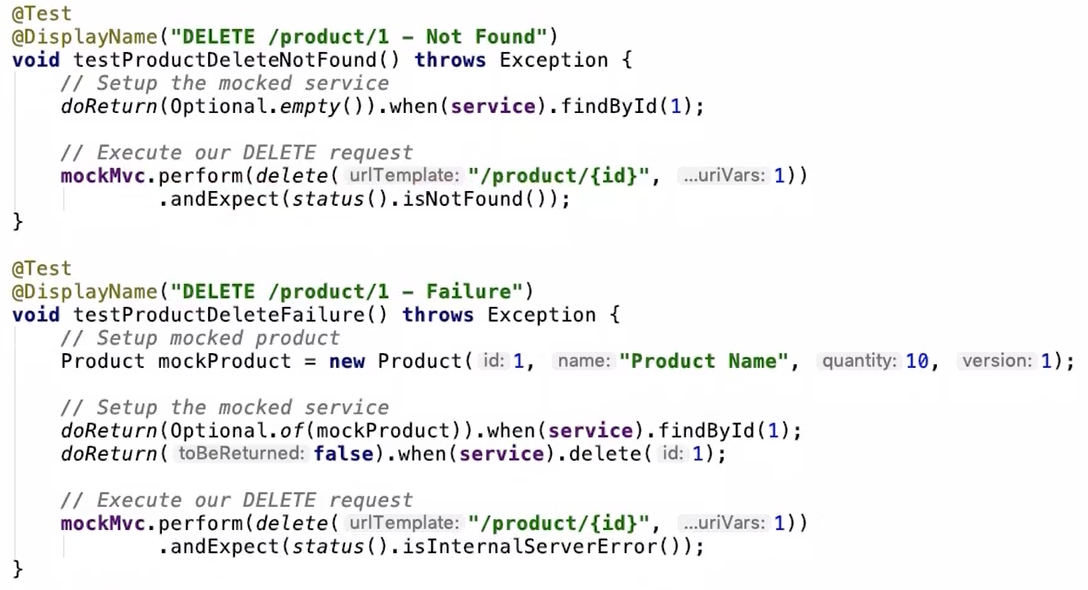
\includegraphics[width=12cm]{img/test_delete_nok.png}
	};
\end{tikzpicture}
\end{frame}

\begin{frame}[fragile]
	\frametitle{Contrôleur DELETE, qui était testé}
	\begin{tikzpicture}[overlay,remember picture]
		\node[anchor=center,xshift=10pt,yshift=0pt]
		at (current page.center) {
			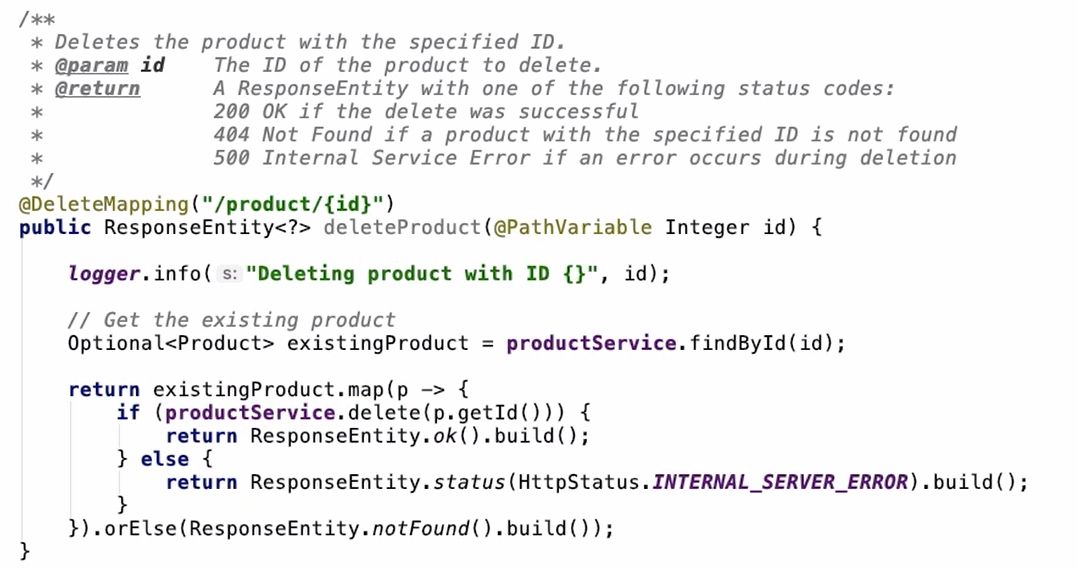
\includegraphics[width=12cm]{img/delete_controller.png}
		};
	\end{tikzpicture}
\end{frame}

\begin{frame}[fragile]
	\frametitle{2. Tester les services}
	\begin{itemize}
		\item Comme vu dans les cours précédents, les services implémentent la logique métier (pour décharger le contrôleur de cette tâche)
		\item Ils servent comme intermédiaire entre les contrôleurs et les repositories
		\item Dans les exemples donnés précédemment, on a 4 méthodes~: \texttt{find}, \texttt{save}, \texttt{update} et \texttt{delete}
	\end{itemize}
\end{frame}

\begin{frame}[fragile]
	\frametitle{Interface du service à tester}
	\begin{tikzpicture}[overlay,remember picture]
		\node[anchor=center,xshift=0pt,yshift=-20pt]
		at (current page.center) {
			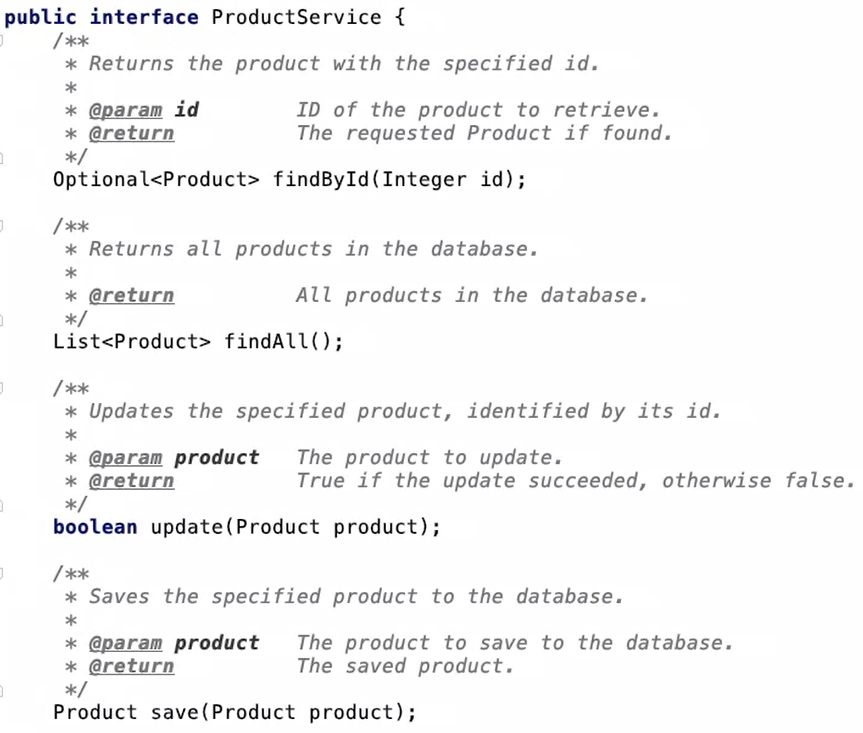
\includegraphics[width=9cm]{img/service_example.png}
		};
	\end{tikzpicture}
\end{frame} 

\begin{frame}[fragile]
	\frametitle{Implémentation du service à tester}
	\begin{tikzpicture}[overlay,remember picture]
		\node[anchor=center,xshift=0pt,yshift=0pt]
		at (current page.center) {
			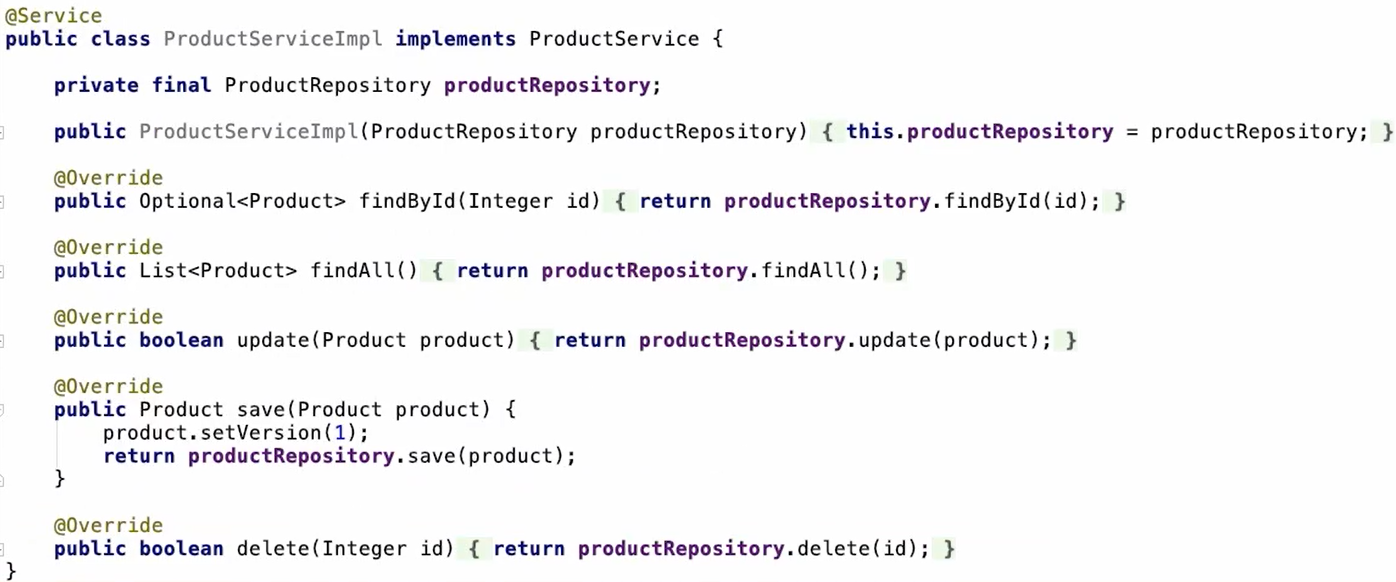
\includegraphics[width=12.5cm]{img/service_impl_example.png}
		};
	\end{tikzpicture}
\end{frame} 

\begin{frame}[fragile]
	\frametitle{Tester le service -- find}
	\begin{tikzpicture}[overlay,remember picture]
		\node[anchor=center,xshift=0pt,yshift=5pt]
		at (current page.center) {
			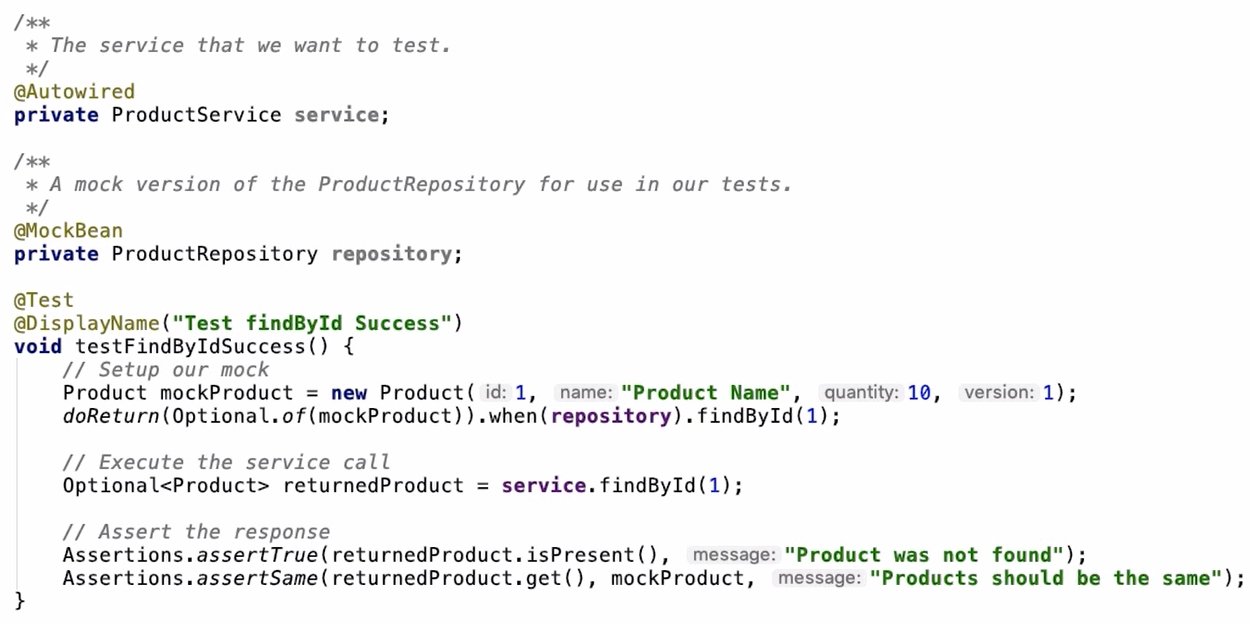
\includegraphics[width=12.5cm]{img/test_service_find.png}
		};
	\end{tikzpicture}
\begin{itemize}
	\vspace{5cm}
	\item Noter l'utilisation du même mécanisme de Mock, mais cette fois pour le repository
	\item On utilise ici des assertions JUnit pour vérifier le résultat
\end{itemize}
\end{frame} 

\begin{frame}[fragile]
	\frametitle{Tester le service -- find Not Found}
	\begin{tikzpicture}[overlay,remember picture]
		\node[anchor=center,xshift=0pt,yshift=5pt]
		at (current page.center) {
			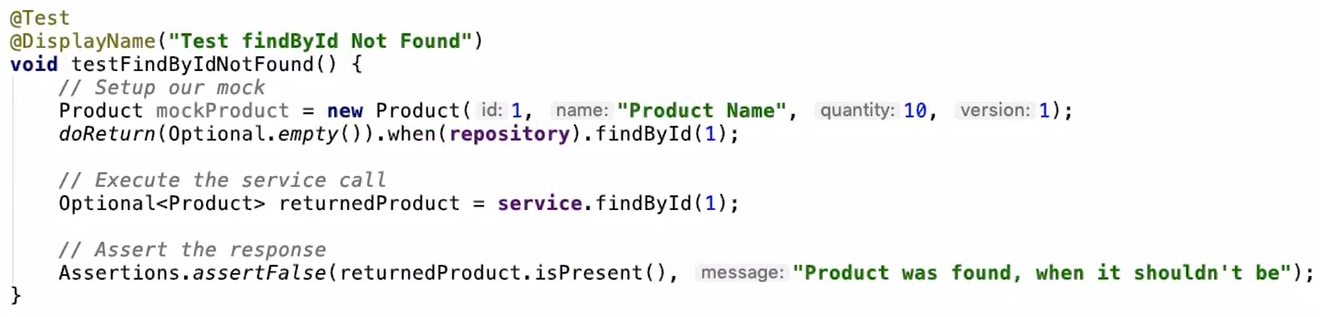
\includegraphics[width=12.5cm]{img/test_service_find_nok.png}
		};
	\end{tikzpicture}
	\begin{itemize}
		\vspace{3cm}
		\item On crée un Mock pour le repository, comme précédemment
		\item On invoque \texttt{findById()} sur le service, comme précédemment
		\item On fait un \texttt{assertFalse()} ici
	\end{itemize}
\end{frame} 

\begin{frame}[fragile]
	\frametitle{Tester le service -- findAll}
	\begin{tikzpicture}[overlay,remember picture]
		\node[anchor=center,xshift=0pt,yshift=20pt]
		at (current page.center) {
			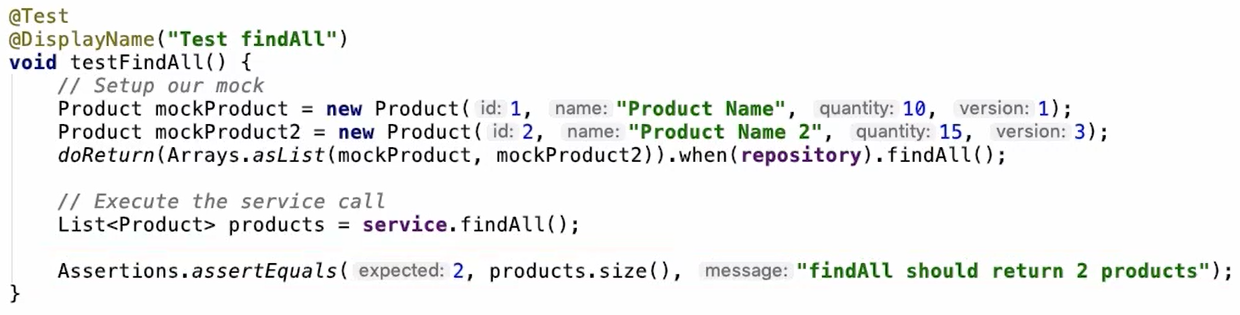
\includegraphics[width=12.5cm]{img/test_service_findAll.png}
		};
	\end{tikzpicture}
	\begin{itemize}
		\vspace{3cm}
		\item On crée un Mock pour le repository, comme précédemment, avec une liste de deux objets simulés
		\item On invoque \texttt{findAll()} sur le service
		\item Enfin, on fait un \texttt{assertEquals()}
	\end{itemize}
\end{frame}


\begin{frame}[fragile]
	\frametitle{Tester le service -- save}
	\begin{tikzpicture}[overlay,remember picture]
		\node[anchor=center,xshift=0pt,yshift=20pt]
		at (current page.center) {
			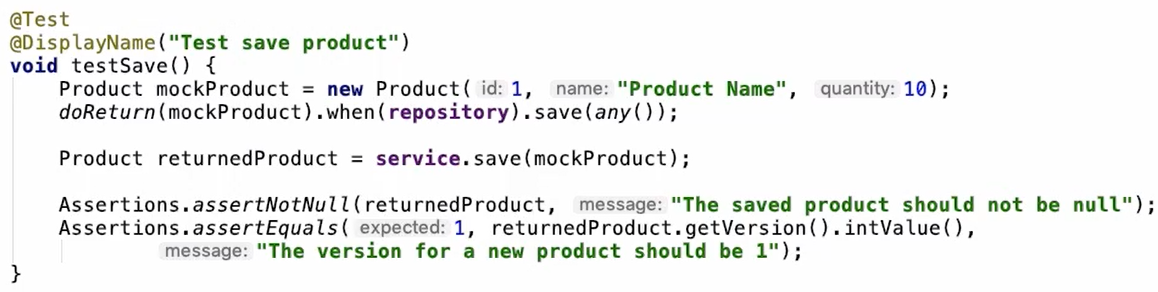
\includegraphics[width=12.5cm]{img/test_service_save.png}
		};
	\end{tikzpicture}
	\begin{itemize}
		\vspace{3cm}
		\item Deux assertions ici. Vérifier que : 1) \texttt{save} retourne un objet et 2) le numéro de version est égal à 1
	\end{itemize}
Il faudrait prévoir aussi des tests pour les autres méthodes (\texttt{update} et \texttt{delete})
\end{frame}

\begin{frame}[fragile]
	\frametitle{3. Tester le repository}
	\begin{itemize}
		\item Dans le repository, méthodes équivalentes à celles du service
		\item Elles interagissent directement avec la BdD
		\item Pour tester un repository (les requêtes SQL), on a le choix entre~:
		\begin{itemize}
			\item Ne pas interagir avec une BdD et utiliser à la place un Mock pour la DataSource~: solution simple et efficace, mais ne permet pas de vérifier concrètement si les requêtes SQL s'exécutent correctement
			\item Tester sur une vraie BdD~: permet de s'assurer que les requêtes SQL sont correctes et si jamais on les change/optimise plus tard, on peut re-tester leur bon fonctionnement
		\end{itemize}
	
	\end{itemize}
	Pour la même raison, on recommande plutôt des tests unitaires pour les repositories et non pas des tests d'intégration
\end{frame}

\begin{frame}[fragile]
	\frametitle{Config dédiée pour tester sur une vraie BdD}
	\begin{itemize}
		\item Il faut mettre en place un environnement de test BdD dédié
		\item On a vu la solution basée sur les profils dans le cours sur Spring Boot (avec un fichier \texttt{application-test.properties})
		\item[] Ce qui est indiqué dans le fichier \texttt{application.properties} sera chargé pour tous les profils	
		\item N'importe quelle classe de bean (annotée \texttt{@Component}, \texttt{@Configuration}, \texttt{@Controller}, ...) peut être annotée \texttt{@Profile("test")} pour limiter sa portée au profil
		\item On a vu dans le cours sur Spring Boot comment on peut activer un profil avec une option de la JVM (-D...). On peut le faire aussi comme paramètre de config Spring Boot~:\\
		\texttt{spring.profiles.active=test}
	\end{itemize}

\end{frame}

\begin{frame}[fragile]
\frametitle{Config dédiée pour tester sur une vraie BdD -suite-}
\begin{itemize}
		\item Souvent, on utilise, pour des raisons de performance, des bases de données \textit{in-memory} pour les tests, comme H2~:
\begin{lstlisting}[language=C]
spring.datasource.driver-class-name=org.h2.Driver
spring.datasource.url=jdbc:h2:mem:db;DB_CLOSE_DELAY=-1
spring.datasource.username=sa
spring.datasource.password=sa
\end{lstlisting}
A déclarer dans un fichier application-test.properties
\item Ensuite, nous allons utiliser DBUnit (framework de tests de bases de données)
\item Nous allons l'utiliser pour créer les tables et insérer des données minimalistes (un dataset de base) et aussi pour rafraîchir/enrichir la BdD à chaque exécution de test 
	\end{itemize}
\end{frame}

\begin{frame}[fragile]
	\frametitle{Concrètement pour utiliser DBUnit}
	\begin{itemize}
		\item Ajouter les dépendances suivantes dans votre script de build Gradle~:
\begin{lstlisting}
testImplementation('org.dbunit:dbunit:2.7.0')
testImplementation('com.github.database-rider:rider-core:1.18.0')
testImplementation('com.github.database-rider:rider-junit5:1.18.0')
testImplementation('com.github.springtestdbunit:spring-test-dbunit:1.3.0')
testImplementation('com.h2database:h2:1.4.200')
\end{lstlisting}
\item Ensuite écrire une classe de tests~:
\begin{lstlisting}
@ExtendWith({DBUnitExtension.class, 
	         SpringExtension.class})
@SpringBootTest
@ActiveProfiles("test")
public class UserRepositoryTest { /* ... */ }
\end{lstlisting}
	\end{itemize}
\end{frame}

\begin{frame}[fragile]
	\frametitle{Concrètement pour utiliser DBUnit -suite-}
	\begin{itemize}
		\item Préparer un fichier Yaml pour le dataset minimal et le stocker comme~: \texttt{src/test/resources/datasets/users.yml}~:
\begin{lstlisting}
users:
 - id: 1
   prenom: "Yan"
   nom: "Brooks"
   age: 47
 - id: 2
   prenom: "Dan"
   nom: "Waynes"
   age: 54
\end{lstlisting}
\item Première ligne~: nom de la table\\
\item Les autres champs doivent correspondre aux champs de la table
	\end{itemize}
\end{frame}

\begin{frame}[fragile]
	\frametitle{Concrètement pour utiliser DBUnit -suite-}
	\begin{itemize}
		\item Définir un fichier \texttt{schema.sql} pour créer la table dans \texttt{src/main/resources}~:
\begin{lstlisting}
CREATE TABLE IF NOT EXISTS users (
id  INTEGER NOT NULL AUTO_INCREMENT,
prenom VARCHAR(30) NOT NULL,
nom VARCHAR(30) NOT NULL,
age INTEGER NOT NULL,
PRIMARY KEY (id)
);
\end{lstlisting}
	\end{itemize}
\end{frame}

\begin{frame}[fragile]
	\frametitle{Concrètement pour utiliser DBUnit -suite-}
	\begin{itemize}
		\item Dans la classe de test ajouter~:
\begin{lstlisting}
@Autowired
private DataSource dataSource;
public ConnectionHolder getConnectionHolder() {
	return () -> dataSource.getConnection();
}
@Autowired
private UserRepository repository;
@Test
@DataSet("users.yml")
void testFindAll() {
 List<User> users = 
            Lists.newArrayList(repository.findAll());
 Assertions.assertEquals(2, users.size(), 
            "Expected 2 users in the database");
}	
\end{lstlisting}
Ici, on teste si findAll retourne bien deux objets (ceux du .yml)
	\end{itemize}

\end{frame}

\begin{frame}[fragile]
	\frametitle{Dans le précédent test}
	\begin{itemize}
		\item Ouvrir sur votre IDE l'annotation DataSet (appui sur Ctrl+l'annotation) pour voir les options possibles~:
		\begin{itemize}
		\item \texttt{value} : dataset à charger
		\item \texttt{strategy} : on a laissé ici la valeur par défaut, qui est \texttt{CLEAN\_INSERT}, qui veut dire effacer et insérer dans la base les données du dataset à chaque exécution du test case
		\item[] Autres valeurs possibles~: \texttt{INSERT} (ajout de façon incrémentale), \texttt{UPDATE} (mettre à jour les données de la base avec le nouveau dataset), ...
		\item On peut également paramétrer cette annotation pour mettre en place des scripts SQL qui s'exécutent avant, après le test, ...

		\end{itemize}
	\end{itemize}
Enfin, on doit ajouter des \textit{tests cases} pour les autres méthodes du repository utilisées dans l'application (cas de succès et échec)
\end{frame}

\section{Tests d'intégration}

\begin{frame}
	\frametitle{Idée générale}
	\begin{itemize}
		\item Tester si tout ce qui a été développé et testé séparément fonctionne bien une fois connecté ensemble
		\item Tester si une fois les contrôleurs, reliés aux services, et les services aux repositories, le tout fonctionne correctement
		\item Pourquoi~?
		\begin{itemize}
			\item Vérifier que la configuration (connexion des composants) est correcte
			\item S'assurer que la fonctionnalité end-to-end (sans le front) marche correctement
		\end{itemize}
	\end{itemize}
\end{frame}

\begin{frame}
	\frametitle{Test d'intégration}
	\begin{tikzpicture}[overlay,remember picture]
		\node[anchor=center,xshift=0pt,yshift=20pt]
		at (current page.center) {
			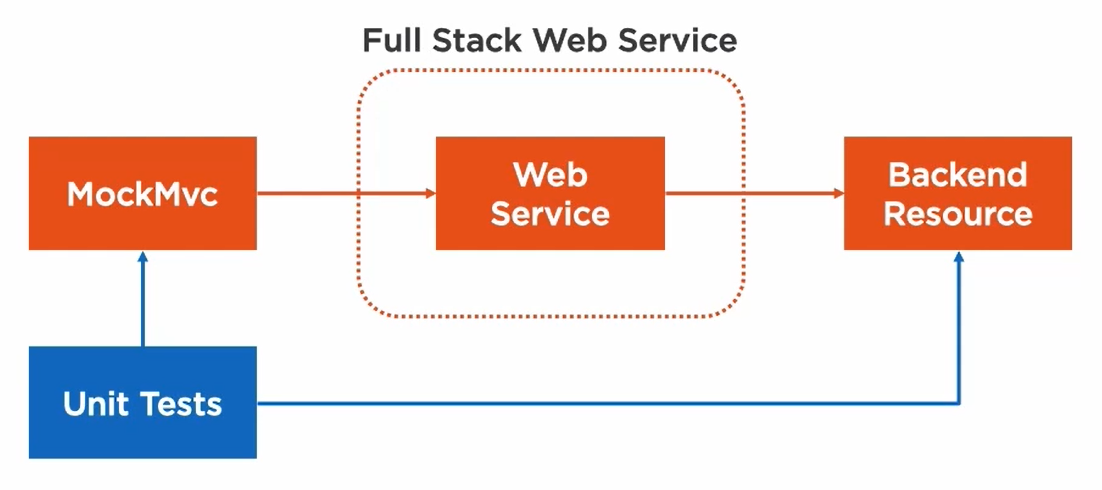
\includegraphics[width=10cm]{img/integration_test.png}
		};
	\end{tikzpicture}
\begin{itemize}
	\vspace{4cm}
	\item Nous utiliserons MockMVC pour éviter le démarrage d'un serveur Web (et simuler des requêtes/réponses HTTP)
	\item Nous utiliserons aussi une BdD in-memory (H2) pour simuler la source de données
\end{itemize}
\end{frame}

\begin{frame}
	\frametitle{Test d'intégration avec MockMvc et H2}
	\begin{tikzpicture}[overlay,remember picture]
		\node[anchor=center,xshift=0pt,yshift=20pt]
		at (current page.center) {
			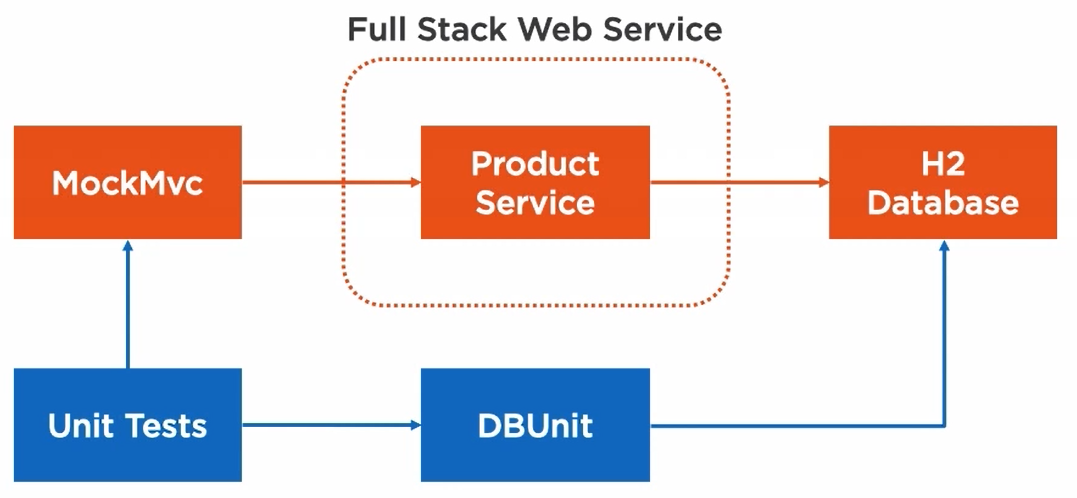
\includegraphics[width=10cm]{img/integration_test_h2.png}
		};
	\end{tikzpicture}
\begin{itemize}
	\vspace{4cm}
	\item Nous utiliserons aussi DBUnit pour tester les repositories
\end{itemize}
	
\end{frame}

\begin{frame}[fragile]
	\frametitle{Classe de test d'intégration}
\begin{lstlisting}
@ExtendWith({DBUnitExtension.class, SpringExtension.class})
@SpringBootTest
@Profile("test")
@AutoConfigureMockMvc
public class UserServiceIntegrationTest {
 @Autowired
 MockMvc mockMvc;
 @Autowired
 private DataSource dataSource;	
 public ConnectionHolder getConnectionHolder() {
  // Return a function that retrieves a connection 
  // from our data source
  return () -> dataSource.getConnection();
 }
 // ...
}
\end{lstlisting}
	\begin{itemize}
		\item Noter l'utilisation de l'attribut auto-injecté MockMvc
	\end{itemize}
\end{frame}

\begin{frame}[fragile]
	\frametitle{Méthode de test d'intégration - Get - Found}
\begin{lstlisting}
@Test
@DisplayName("GET /user/1 - Found")
@DataSet("users.yml")
void testGetUserByIdFound() throws Exception {
 // Execute the GET request
 mockMvc.perform(get("/user/{id}",1))
 // Validate the status code and content type
 .andExpect(status().isOk())
 .andExpect(content().contentType(MediaType.APPLICATION_JSON))
 // Validate the returned fields
 .andExpect(jsonPath("$.id"),is(1))
 .andExpect(jsonPath("$.prenom"),is("Yan"))
 .andExpect(jsonPath("$.nom"),is("Brooks"))
 .andExpect(jsonPath("$.age"),is(47));
}
\end{lstlisting}
\end{frame}

\begin{frame}[fragile]
\frametitle{Méthode de test d'intégration - imports}

	\begin{itemize}
		\item Prévoir les imports statiques suivants~:
\begin{lstlisting}
import static org.springframework.test.web.servlet.request.MockMvcRequestBuilders.*;
import static org.springframework.test.web.servlet.result.MockMvcResultMatchers.*;
import static org.springframework.test.web.servlet.result.MockMvcResultHandlers.*;
import static org.mockito.Mockito.*;
import static org.hamcrest.Matchers.*;
\end{lstlisting}
	\end{itemize}
\end{frame}

\begin{frame}[fragile]
	\frametitle{Méthode de test d'intégration - Get - Not Found}
\begin{lstlisting}
@Test
@DisplayName("GET /user/99 - Not Found")
@DataSet("users.yml")
void testGetUserByIdNotFound() throws Exception {
 // Execute the GET request
 mockMvc.perform(get("/user/{id}",99))
 // Validate the status code and content type
 .andExpect(status().isNotFound());
}
\end{lstlisting}
\end{frame}

\begin{frame}[fragile]
	\frametitle{Méthode de test d'intégration - Post - Success}
\begin{lstlisting}
@Test
@DisplayName("POST /user - Success")
@DataSet("users.yml")
void testCreateUser() throws Exception {
 // Setup User to create
 String prenom="Lisa", nom="Holmes"; int age=26;
 User user = new User(prenom,nom,age);
 // Execute the POST request
 mockMvc.perform(post("/user")
 .contentType(MediaType.APPLICATION_JSON)
 .content(asJsonString(user)))
 // Validate the status code and content type
 .andExpect(status().isCreated()).andExpect(
   content().contentType(MediaType.APPLICATION_JSON))
 // Validate the returned fields
 .andExpect(jsonPath("$.id",is(3)))
 .andExpect(jsonPath("$.prenom",is(prenom)))
 .andExpect(jsonPath("$.nom",is(nom)))
 .andExpect(jsonPath("$.age",is(age))); }
\end{lstlisting}
\end{frame}

\begin{frame}[fragile,label={obj2json}]
	\frametitle{Méthode de test d'intégration - sérialisation}
\begin{lstlisting}
private String asJsonString(Object obj) {
 try {
  return new ObjectMapper().writeValueAsString(obj);
 } catch (IOException e) {
  throw new RuntimeException(e);
 }
}
\end{lstlisting}
Prévoir enfin des méthodes de test pour les autres opérations du service~:
\begin{itemize}
	\item mise à jour d'un user (put), avec succès, conflit, not found
	\item suppression d'un user (delete), avec succès, not found
\end{itemize}

\end{frame}

\begin{frame}
	\frametitle{Conclusion}
	\begin{itemize}
		\item Tests automatiques très importants dans le développement d'une application Web
		\item Aident à vérifier le comportement correct de l'application
		\item Font qu'on peut faire des changements sans avoir peur de casser l'application
		\item TDD (\textit{Test-Driven Development})~: écrire d'abord les tests, qui échouent tous au départ, et ensuite développer l'application pour faire passer les tests au vert l'un après l'autre (paradigme un peu lent au départ, mais développement sûr)
		\item Spring offre plein de facilités pour écrire des tests, en intégrant de façon transparente/facile plusieurs autres frameworks JUnit, Mockito, Hamcrest, ...
	\end{itemize}
\end{frame} 

\begin{frame}
	\frametitle{Conclusion -suite- et références biblio}
	\begin{itemize}
		\item Pour aller plus loin (``\textit{out of scope}" de ce cours), faire les tests end-to-end en intégrant le front, avec des frameworks comme Cypress (\url{https://www.cypress.io/})~: tester les interfaces utilisateurs, les navigations, les vérifier et ensuite rejouer cela à chaque changement dans l'application
	\end{itemize}
	Références biblio~:
	\begin{itemize}
		\item Site Web de Spring Testing~: \url{https://spring.io/guides/gs/testing-web/}
		\item Tutoriels sur Pluralsight et Baeldung
	\end{itemize}
\end{frame} 


\begin{frame}
	\begin{tikzpicture}[overlay,remember picture]
		\node[anchor=center,xshift=0pt,yshift=0pt]
		at (current page.center) {
			
\includegraphics[width=4cm]{img/question.jpg}
		};
	\end{tikzpicture}
\end{frame}

\end{document}
